\section{Visualisierung mit Manim}

Ziel dieses Kapitels war es, das anamorphotische Distanzpunktverfahren nach Niceron algorithmisch in Manim zu implementieren. Dafür wurde ein objektorientierter Ansatz in Python gewählt, mit dem hochauflösende Phasenbilder für jede einzelne Konstruktionsphase generiert wurden.

In den ersten beiden Konstruktionsschritten (vgl. Abb. 1a und 1b) etabliert das Skript das räumliche Fundament und die Tiefenlinien. Hierzu werden der Hauptfluchtpunkt $P(0,3)$ und der Distanzpunkt $D(4,3)$ in einem diskreten Koordinatensystem definiert. Anschließend generiert eine iterative Schleife die orthogonalen Tiefenlinien, welche alle im Hauptfluchtpunkt konvergieren. 

In den Phasen 3 und 4 (vgl. Abb. 1c und 1d) wird zunächst ausgehend vom linken Rand der Grundlinie $L(-5,-4)$ eine Diagonale zum Distanzpunkt $D$ gezogen. Mithilfe einer weiteren Schleife und der algebraischen Berechnung der Variablen $y_{pos}$ und $x_r$ zeichnet der Algorithmus die horizontalen Querlinien in den exakt berechneten, perspektivisch korrekten Höhen ein. Um das Raster schließlich zu verzerren, nutzt das Skript ein Sampling-Verfahren. Dabei wird jede Gerade der ursprünglichen Form in eine äquidistante Anzahl von Punkten unterteilt. Diese werden Punkt für Punkt durch die Transformationsfunktion berechnet und zu einem geschlossenen, anamorphotisch verzerrten Polygon verbunden. 

Auf die Implementierung eines allgemeineren Verfahrens, welches beliebige Objekte korrekt anamorphotisch darstellt, wurde hierbei bewusst verzichtet, um das klassische Konstruktionsverfahren nach Niceron didaktisch klar und nachvollziehbar zu vermitteln.

\begin{figure}[htbp]
    \centering
    % Erste Reihe
    \begin{subfigure}[t]{0.48\textwidth}
        \centering
        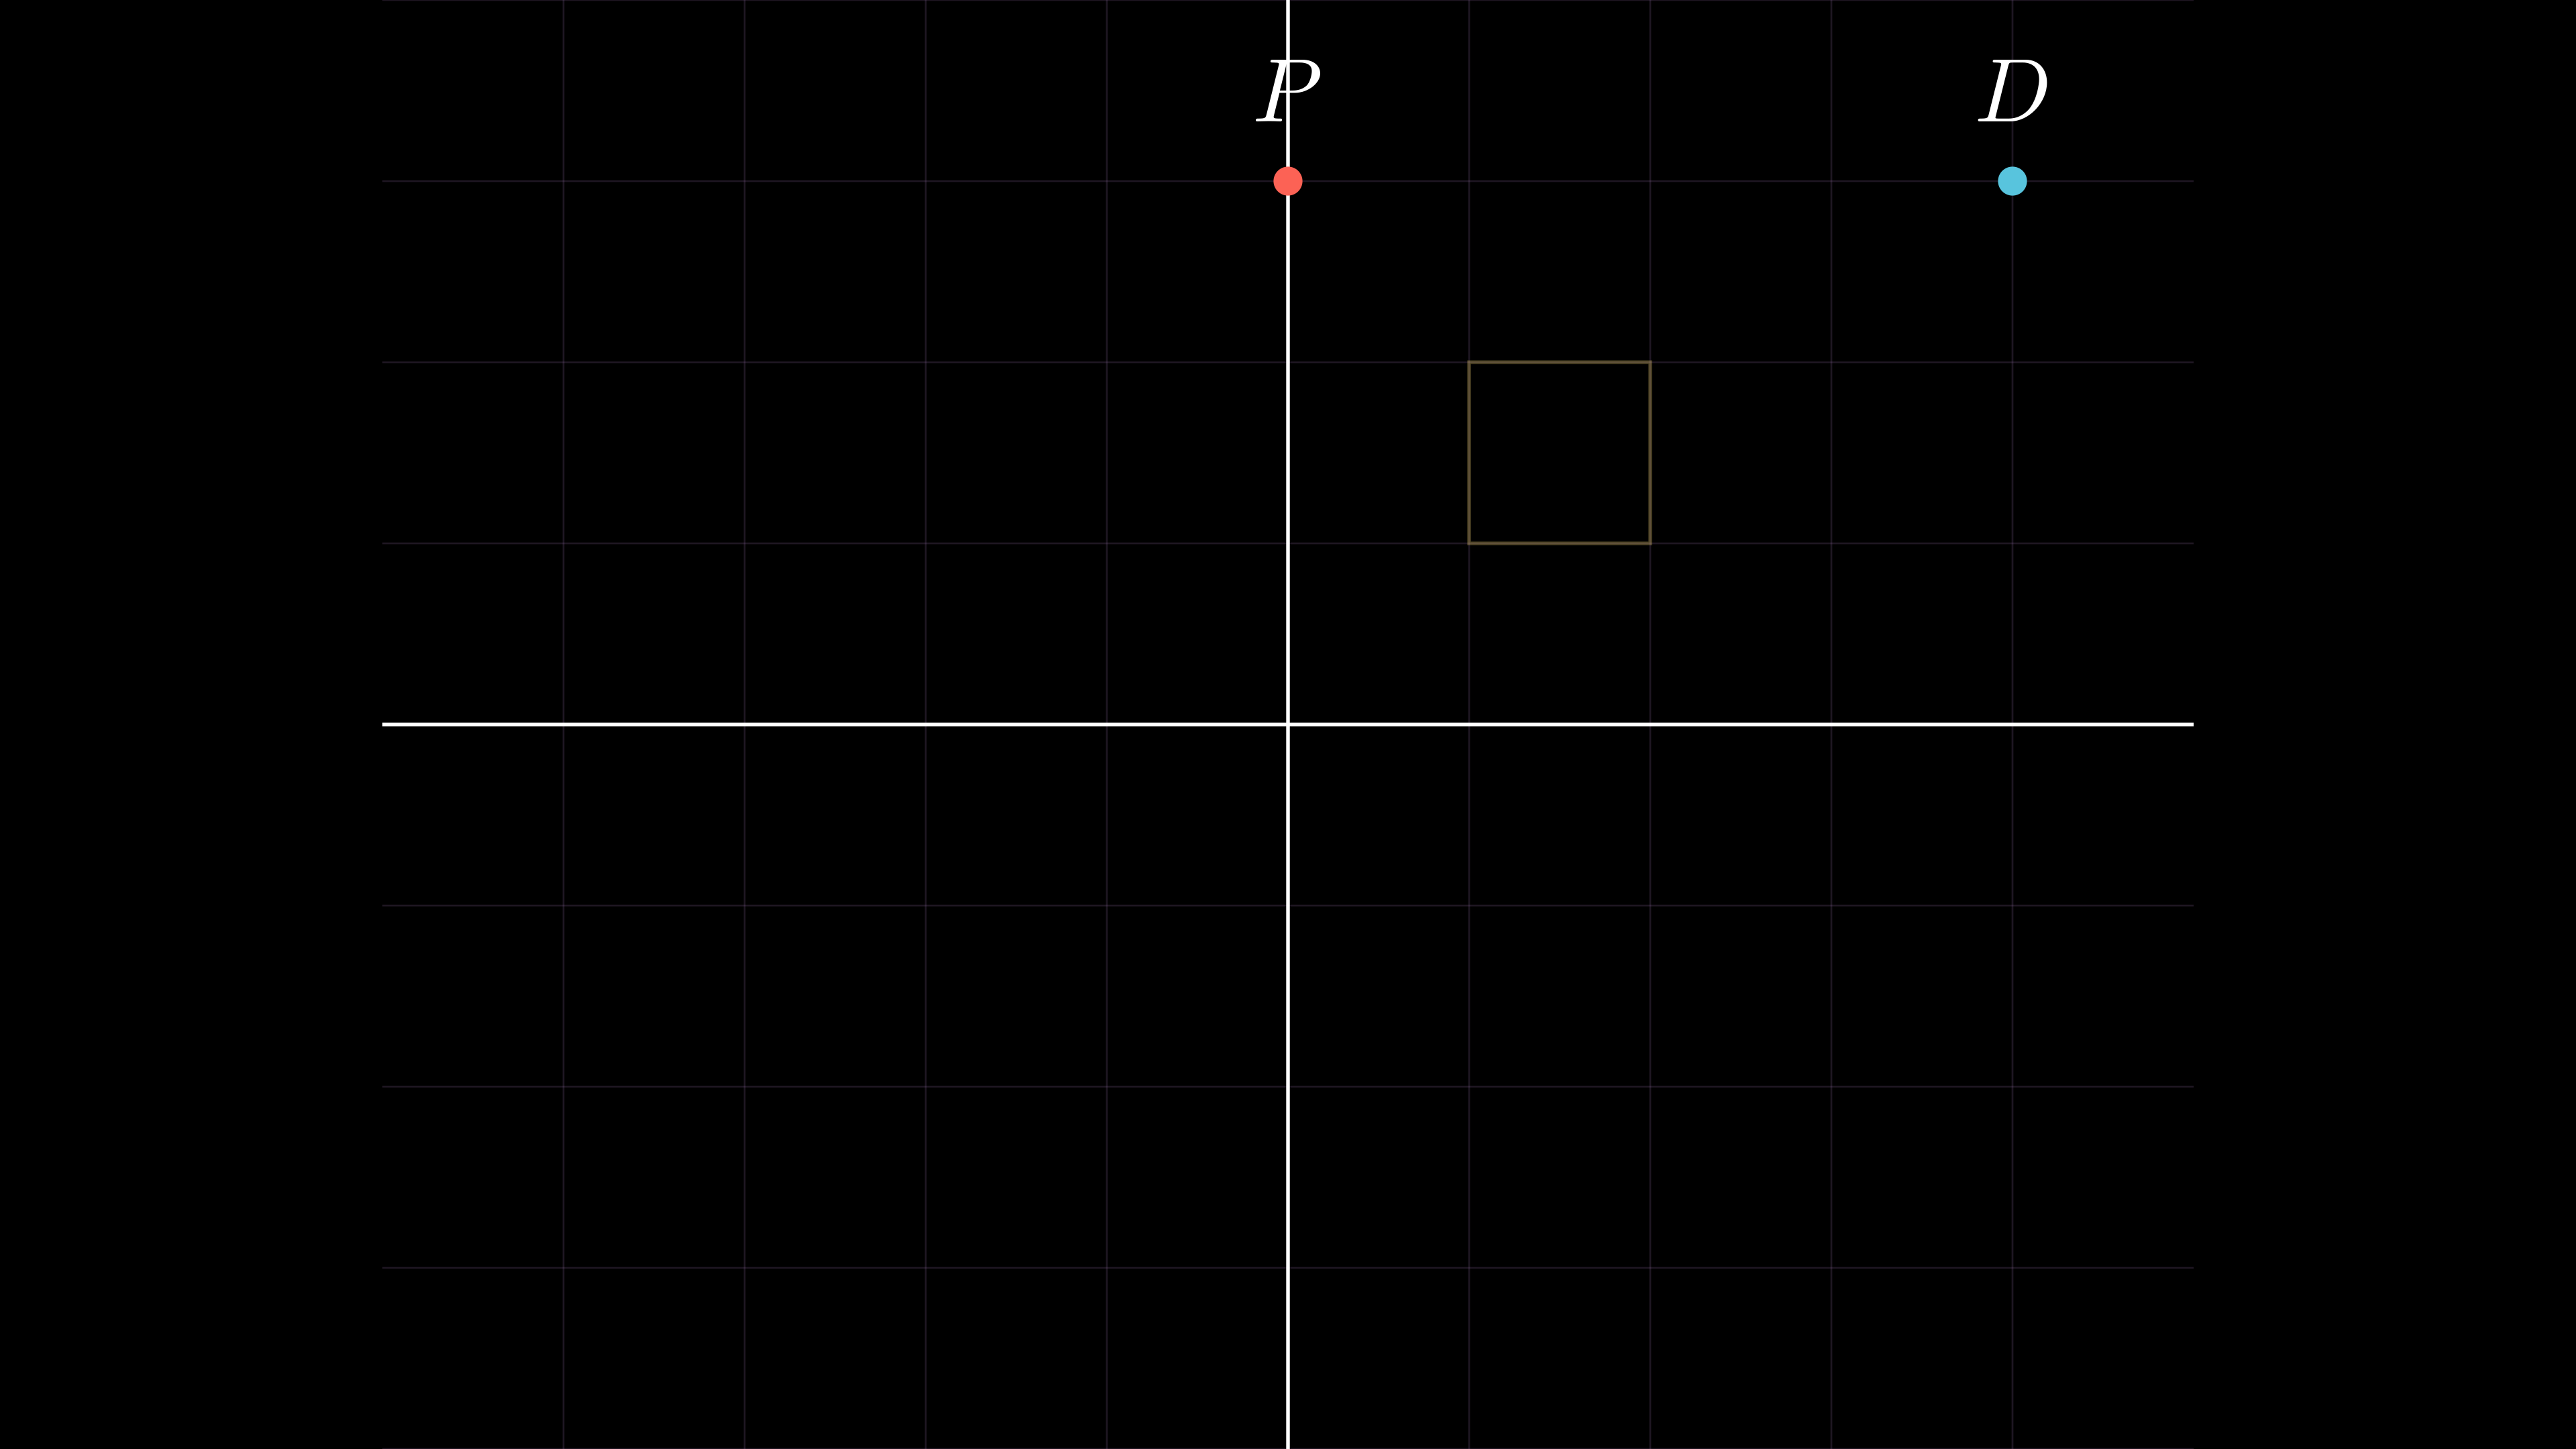
\includegraphics[width=\textwidth]{img/Phase1.png}
        \caption{Phase 1: Das reguläre, unverzerrte Grundraster.}
        \label{fig:phase1}
    \end{subfigure}
    \hfill
    \begin{subfigure}[t]{0.48\textwidth}
        \centering
        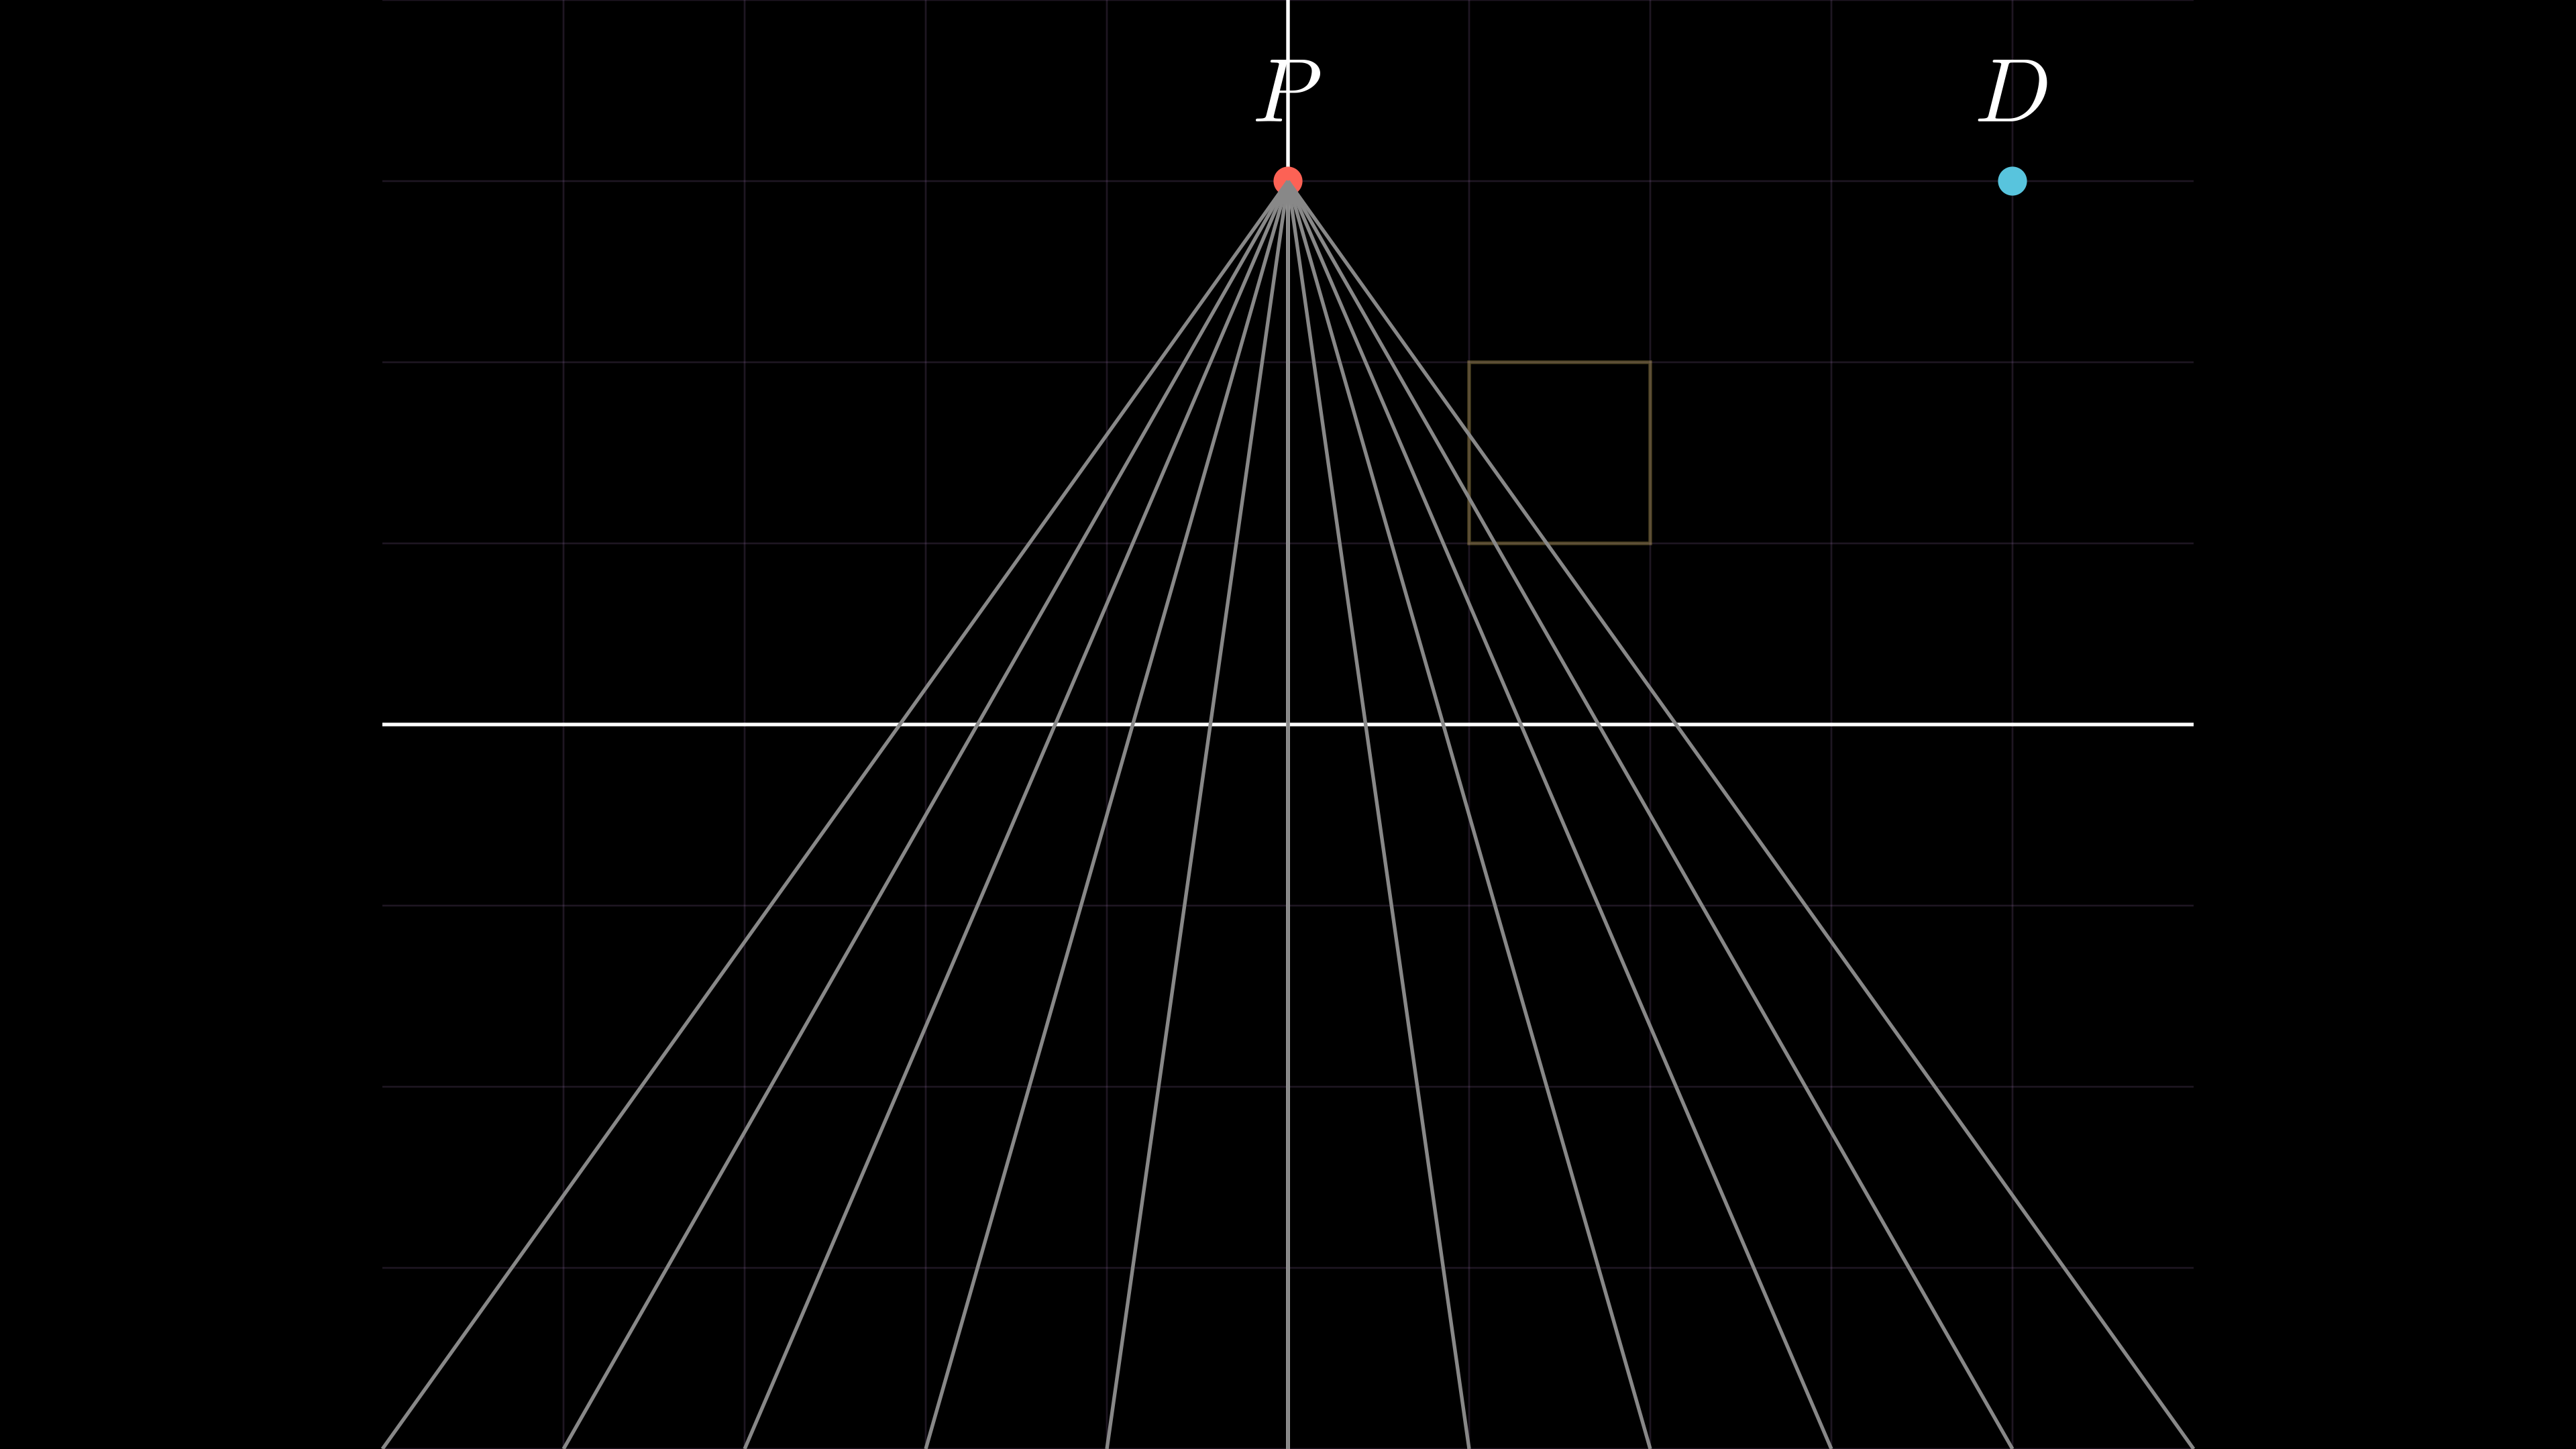
\includegraphics[width=\textwidth]{img/Phase2.png}
        \caption{Phase 2: Hauptfluchtpunkt und Distanzpunkt zur Tiefenbestimmung.}
        \label{fig:phase2}
    \end{subfigure}
    
    \vspace{0.5cm} % Abstand zwischen den Reihen
    
    % Zweite Reihe
    \begin{subfigure}[t]{0.48\textwidth}
        \centering
        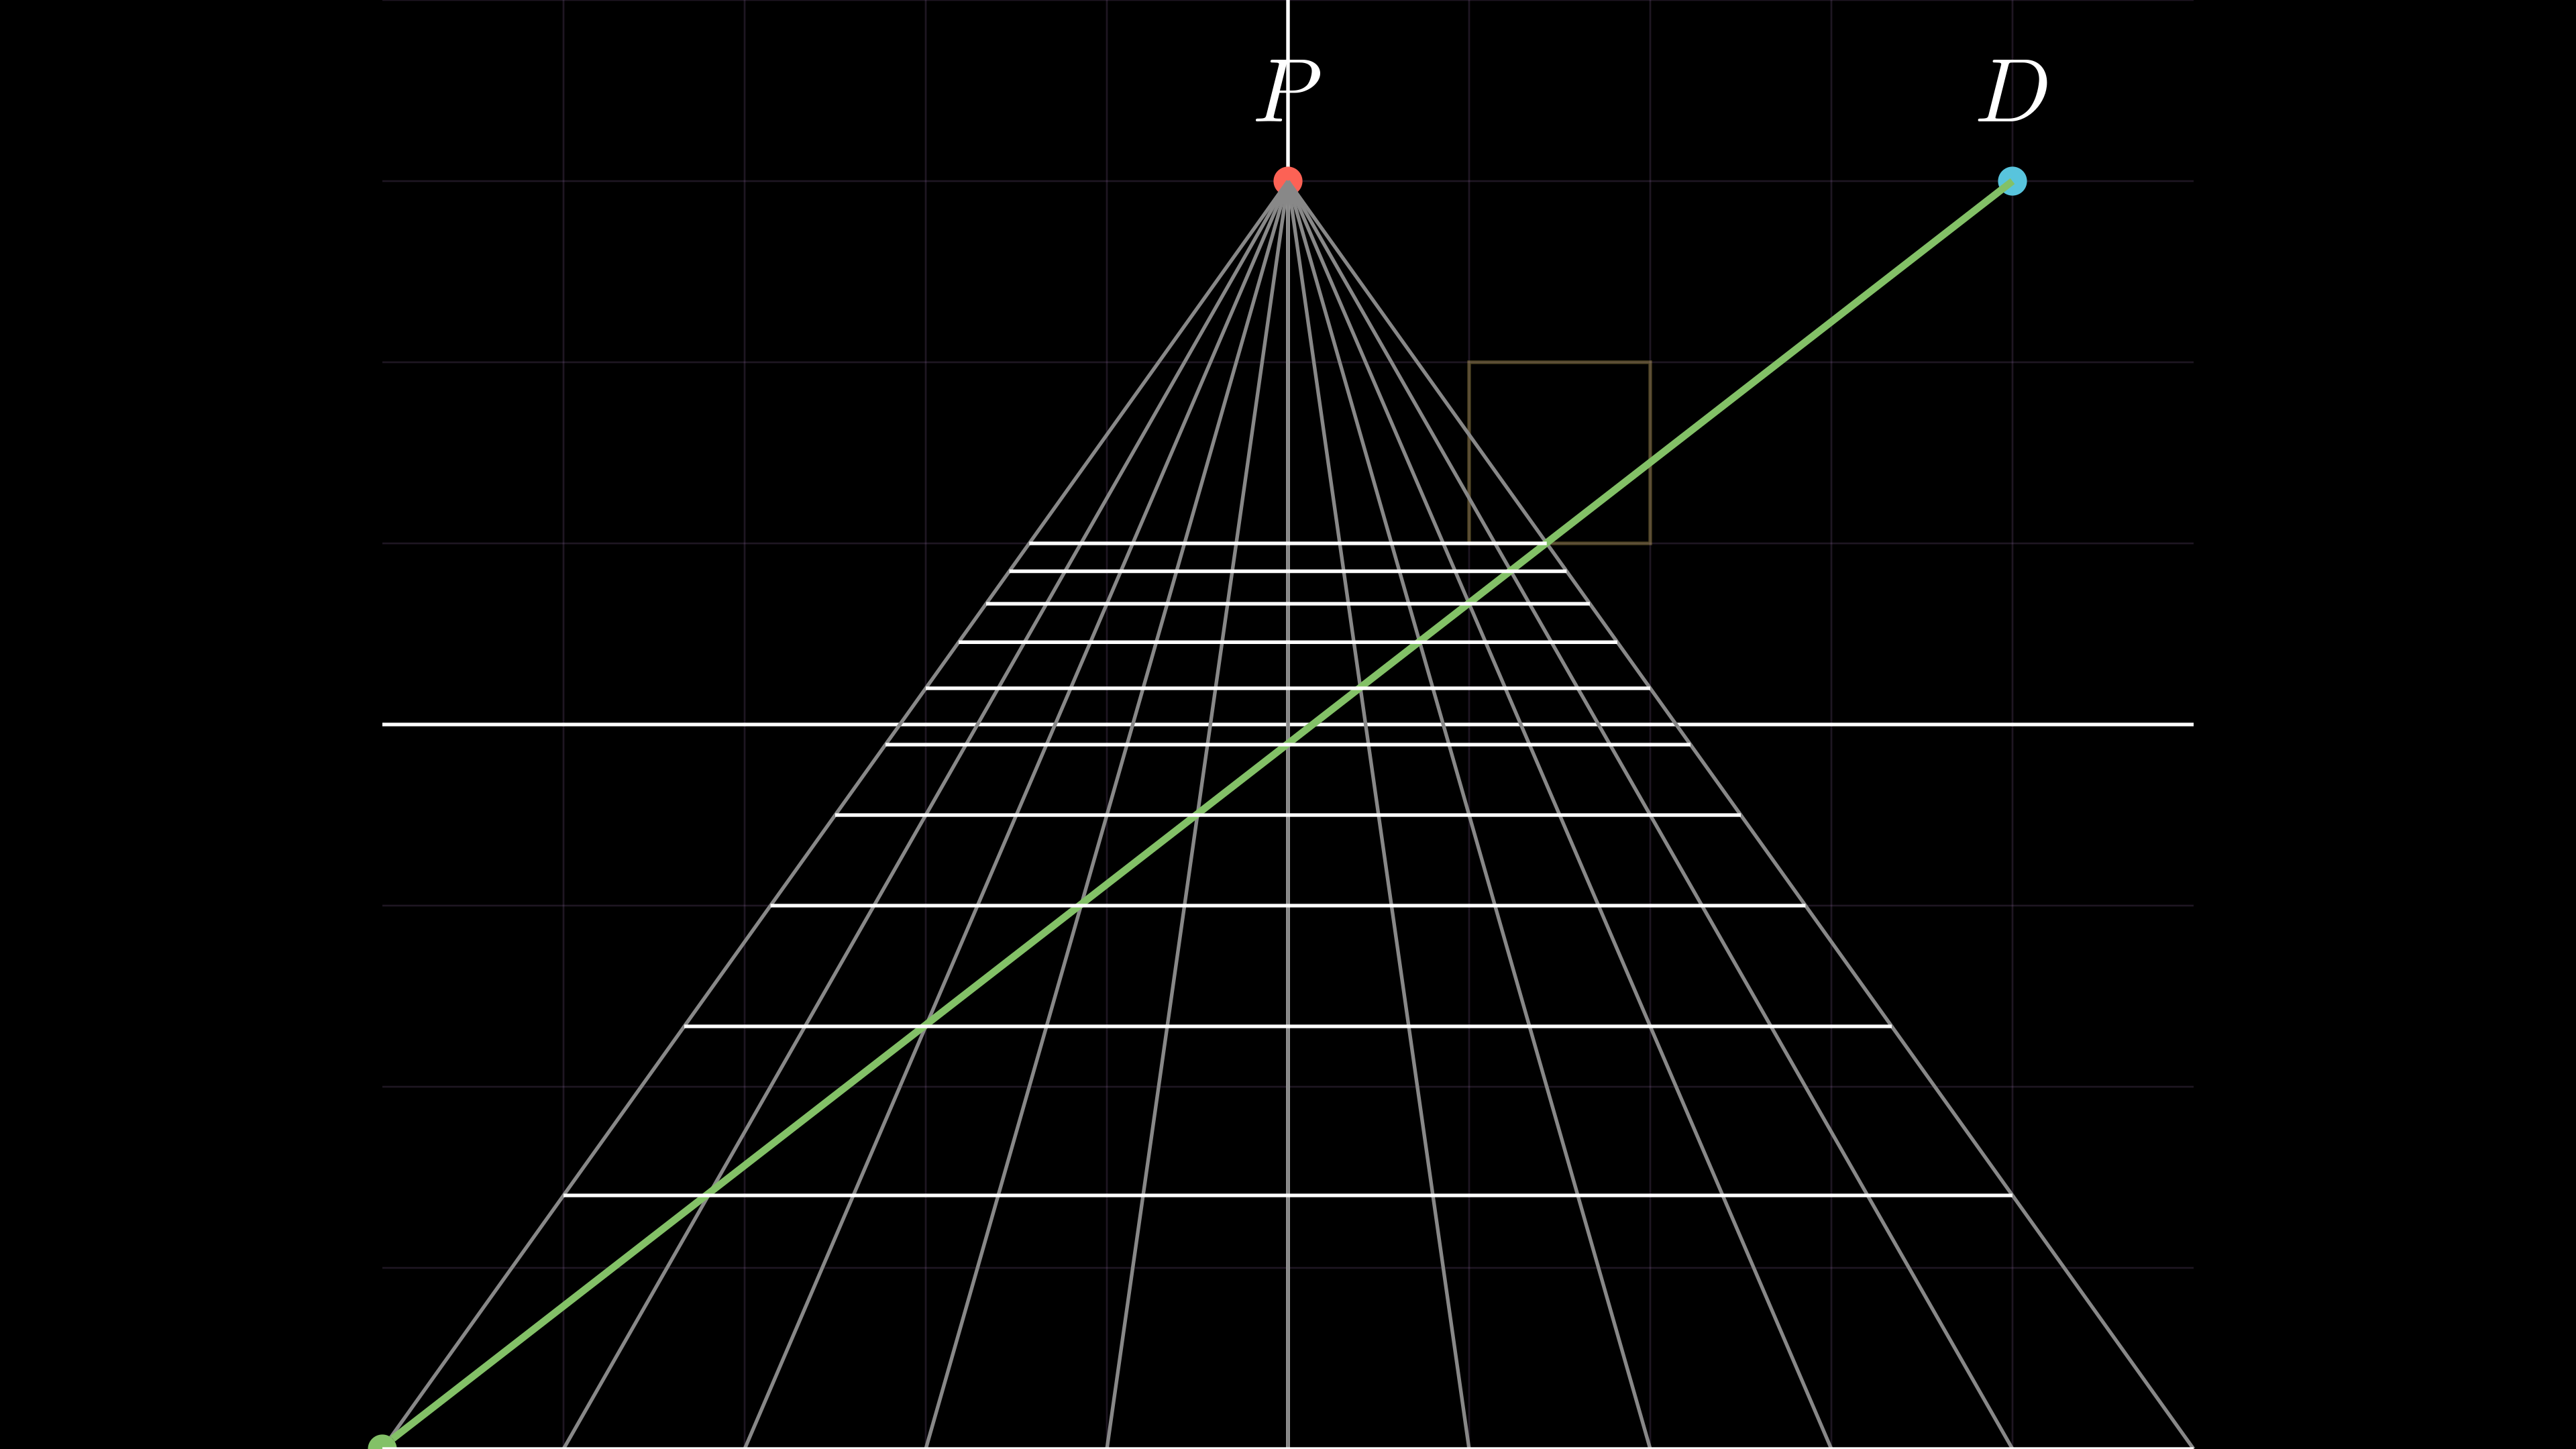
\includegraphics[width=\textwidth]{img/Phase3.png}
        \caption{Phase 3: Projektion der 45$^\circ$-Diagonalen für die Querlinien.}
        \label{fig:phase3}
    \end{subfigure}
    \hfill
    \begin{subfigure}[t]{0.48\textwidth}
        \centering
        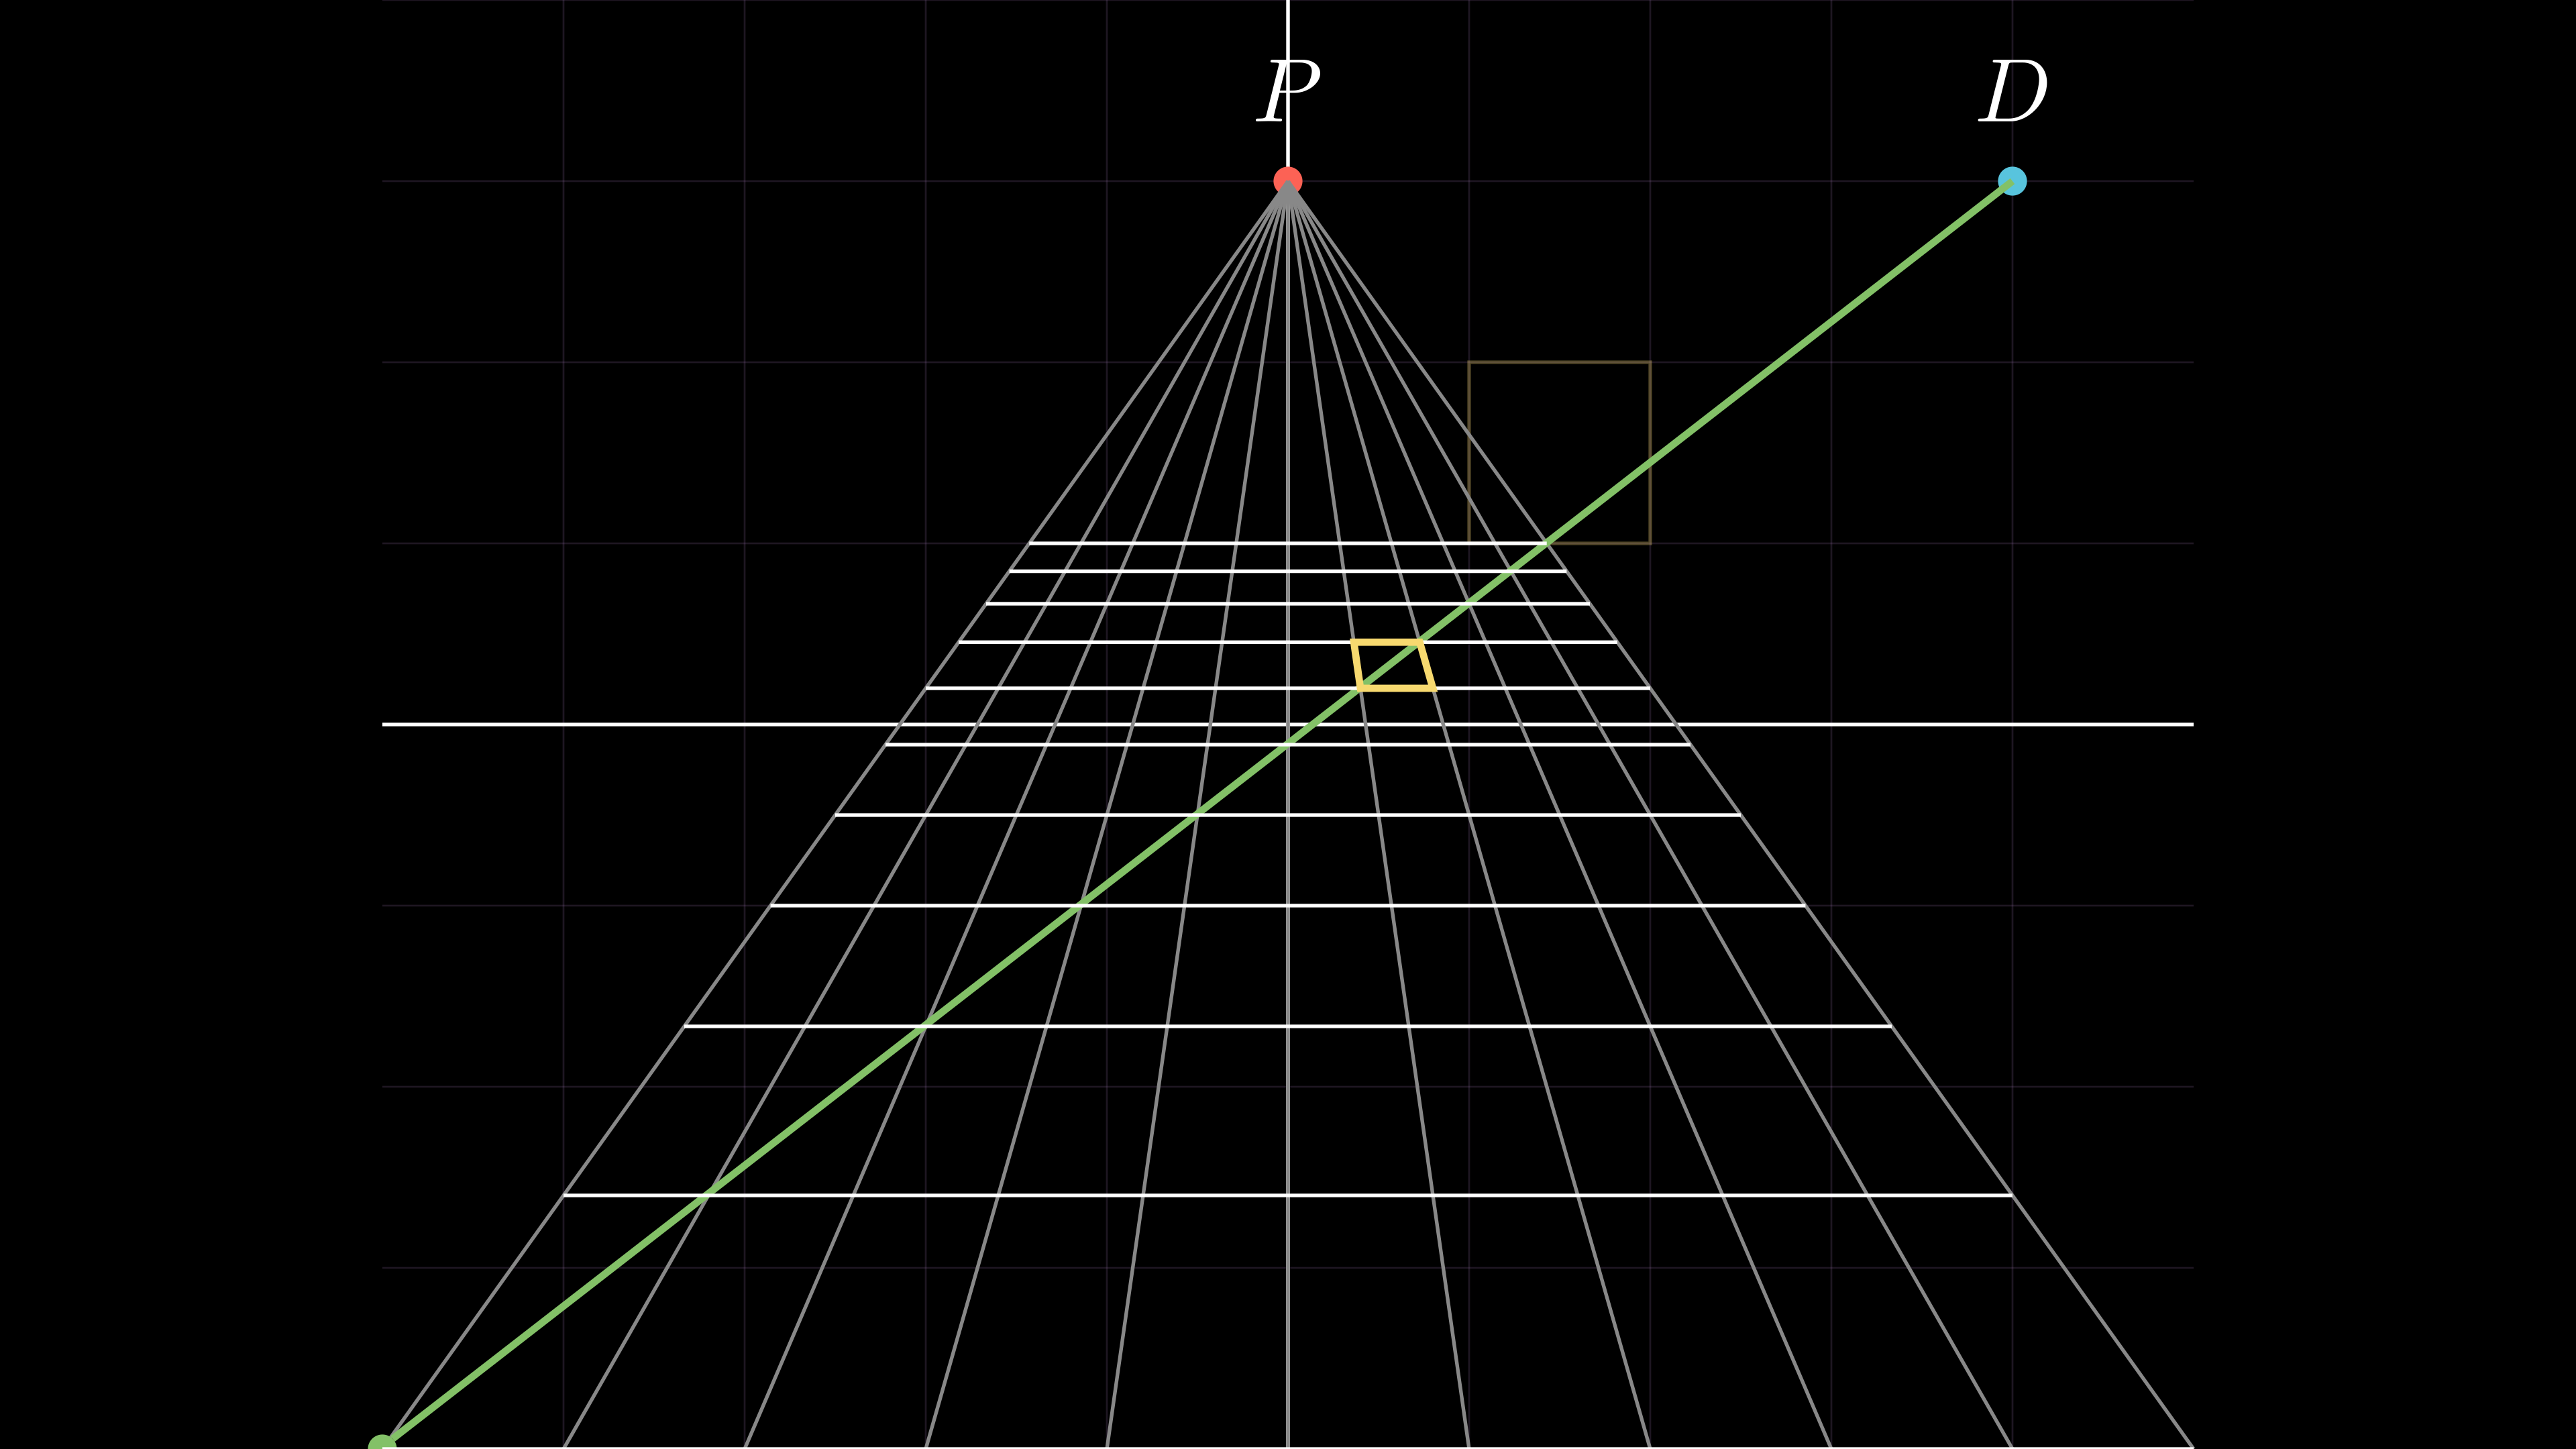
\includegraphics[width=\textwidth]{img/Phase4.png}
        \caption{Phase 4: Das finale, anamorphotisch verzerrte Netz.}
        \label{fig:phase4}
    \end{subfigure}
    
    \caption{Algorithmische Konstruktion der anamorphotischen Projektion nach Niceron mittels Manim.}
    \label{fig:manim_phasen}
\end{figure}

% Hier der Befehl zum direkten Einlesen der Datei
%\lstinputlisting[language=Python, caption={Manim Implementierung}, label={lst:manim_code}]{code/raster.py}